\documentclass{beamer}

\renewcommand{\arraystretch}{1.5}
\usepackage{graphicx}
\usepackage{booktabs}\title[Chiselizing SDR Blocks]{Chiselizing SDR Blocks}
\newcommand{\gwidth}[0]{0.7\textwidth}
\author{Albert Magyar}
\date{\today}

\begin{document}
\begin{frame}
  \titlepage
  \begin{figure}
    \centering
    \includegraphics[width=\gwidth]{figs/chisel.svg}
  \end{figure}
\end{frame}

\begin{frame}{Why we're excited}
  \begin{itemize}
  \item RFNoC shares many of our goals
    \begin{itemize}
    \item High-level system design
    \item Hardware-software integration
    \end{itemize}
  \item Interesting applications in SDR
    \begin{itemize}
    \item Chisel is great for DSP
    \color{blue}\item<2-> Build our external user base!\color{black}
    \end{itemize}
  \end{itemize}
\end{frame}

\begin{frame}{Goals for Chisel on the USRP}
  % Describe ``Chisel SDK''
  Release a Chisel SDK for USRP users
  \begin{itemize}
  \item Allow for a smooth transition from Verilog
  \item Provide a library of common components
  \item Support easy integration with Verilog ecosystem
  \item Increase user productivity!
  \end{itemize}
  \begin{figure}
    \centering
    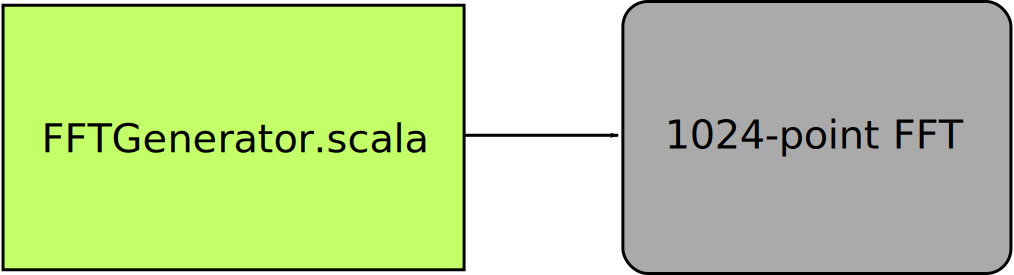
\includegraphics[width=\gwidth]{figs/fftgen.svg}
  \end{figure}
\end{frame}

\begin{frame}{The target: addsub block}
  % block diagram of addsub here
  \begin{figure}
    \centering
    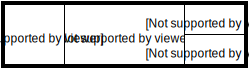
\includegraphics[width=\gwidth]{figs/addsub.svg}
  \end{figure}
\end{frame}

\begin{frame}[fragile]{Step 1: Porting Verilog}
  % can do a rote port without too much of a learning curve
  \begin{itemize}
  \item Simple ports are easy
  \item No Scala magic
  \item Familiar RTL semantics
  \end{itemize}
  \vspace*{5mm}
  \begin{tabular}{ | l | l | }
    \hline
    Verilog & Chisel \\ \hline \small
    \begin{minipage}{0.4\textwidth}
\begin{verbatim}

if (en && incr)
  count <= count + 1;
else if (en && decr)
  count <= count - 1;
...

\end{verbatim}
    \end{minipage} &
    \begin{minipage}{0.5\textwidth}
\begin{verbatim}

when (en && incr) {
  count := count + 1
} .elsewhen (en && decr) {
  count := count - 1
...

\end{verbatim}
    \end{minipage} \\ \hline
  \end{tabular}
  \normalsize
\end{frame}

\begin{frame}{Step 1: Porting Verilog}
  \begin{center}
    \textit{Code Example}
  \end{center}
\end{frame}

\begin{frame}{Interfacing with Verilog}
  % Blackboxes
  \begin{figure}
    \centering
    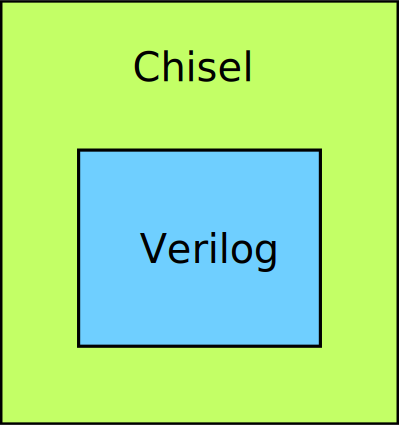
\includegraphics[width=0.5\textwidth]{figs/v_in_c.svg}
  \end{figure}
  \begin{itemize}
    \item Easily accomplished using \texttt{Blackbox} class
    \item Used in research tapeouts
  \end{itemize}
\end{frame}

\begin{frame}{Interfacing with Verilog}
  % Matching port names
  \begin{figure}
    \centering
    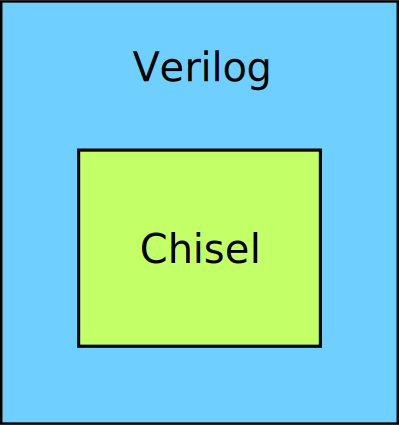
\includegraphics[width=0.5\textwidth]{figs/c_in_v.svg}
  \end{figure}
  \begin{itemize}
    \item Chisel backend produces Verilog
    \item Net names can be coerced with \texttt{setName}
  \end{itemize}
\end{frame}

\begin{frame}{Interfacing with Verilog}
  \begin{center}
    \textit{Verilog Generation Example}
  \end{center}
\end{frame}

\begin{frame}{Interfacing with Verilog: no limits}
  % Matching port names
  \begin{figure}
    \centering
    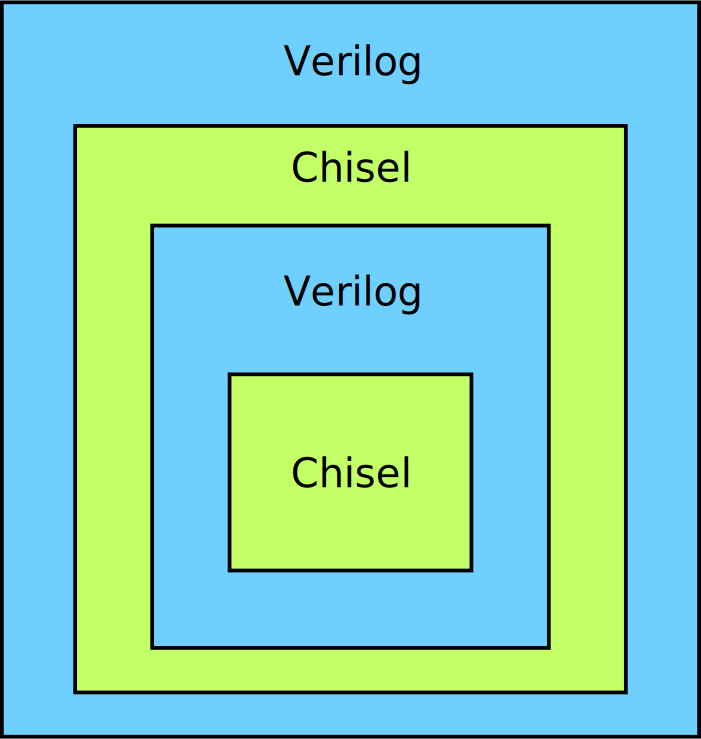
\includegraphics[width=0.5\textwidth]{figs/layers.svg}
  \end{figure}
  \begin{itemize}
    \item In practice, 3 layers has been used
    \item Verilog $<$ Chisel $<$ Verilog
  \end{itemize}
\end{frame}

\begin{frame}{Step $N$: Getting the most from Chisel}
  % Using high-level features productively
  \begin{itemize}
  \item Chisel has helped us define systems at every level
    \begin{itemize}
      \item Reusability \& flexibility in low-level RTL
      \item Defining large systems on a chip
      \item Producing research prototypes
    \end{itemize}
  \item How can we apply Chisel-isms to \texttt{addsub}?
    \begin{itemize}
      \item Rid code of boilerplate
      \item Use parameters for flexible reuse
    \end{itemize}
  \end{itemize}
\end{frame}

\begin{frame}[fragile]{Step $N$: Getting the most from Chisel}
  \small
\begin{verbatim}
class AddSubComplex(dataWidth: Int = 16) extends Module {
  val io = new AddSubComplexIO(dataWidth)
  val sum_q = Module(new Queue(Sample(dataWidth),16))
  val diff_q = Module(new Queue(Sample(dataWidth),16))

  sum_q.io.enq.bits := io.i0.bits + io.i1.bits
  diff_q.io.enq.bits := io.i0.bits - io.i1.bits
  SyncDecoupled(GroupDecoupled(io.i0,io.i1),
    GroupDecoupled(sum_q.io.enq,diff_q.io.enq))

  io.sum.bits := sum_q.io.deq.bits
  io.diff.bits := diff_q.io.deq.bits
  SyncDecoupled(GroupDecoupled(sum_q.io.deq,diff_q.io.deq),
    GroupDecoupled(io.sum,io.diff))
}
\end{verbatim}
\normalsize
\end{frame}

\begin{frame}[fragile]{``On the wire'' types}
  % Reuse: not just modules or verilog functions
  \small
\begin{verbatim}
class AddSubComplexIO(dataWidth: Int = 16) extends Bundle {
  val i0 = new DecoupledIO(Sample(dataWidth)).flip
  val i1 = new DecoupledIO(Sample(dataWidth)).flip
  val sum = new DecoupledIO(Sample(dataWidth))
  val diff = new DecoupledIO(Sample(dataWidth))
}

class AddSubComplex(dataWidth: Int = 16) extends Module {
  ...
  val sum_q = Module(new Queue(Sample(dataWidth),16))
\end{verbatim} 
\normalsize
  \begin{itemize}
  \item Can define arbitrary signal types
    \begin{itemize}
    \item \texttt{DecoupledIO}: generic FIFO interface
    \item \texttt{Sample}: complex number, \texttt{last} bit
    \end{itemize}
  \item Allows for generic modules!
  \end{itemize}
\end{frame}

\begin{frame}{Programmatically constructing circuit graphs}
  % Reuse: not just modules or verilog functions
  It's hard to package RTL as reusible pieces!
  \begin{itemize}
  \item Modules constrain users to rigid portlists
  \item Verilog functions are very limited
  \item Biggest danger: overhead of packaging a module deters designers!
  \end{itemize}
  \vspace*{10mm}
  Chisel allows \textit{explicit} access to circuit graph
  \begin{itemize}
  \item Pointers to nets can be passed around
  \item Functions in Chisel perform any specific graph manipulation
  \item Modularize with or without ``modules''
  \end{itemize}
\end{frame}

\begin{frame}{Programmatically constructing circuit graphs}
  % Reuse: not just modules or verilog functions
  It's hard to package RTL as reusible pieces!
  \begin{itemize}
  \item Modules constrain users to rigid portlists
  \item Verilog functions are very limited
  \end{itemize}
  \vspace*{10mm}
  Chisel allows \textit{explicit} access to circuit graph
  \begin{itemize}
  \item Pointers to nets can be passed around
  \item Functions in Chisel perform any specific graph manipulation
  \end{itemize}
\end{frame}

\begin{frame}[fragile]{Programmatically constructing circuit graphs}
  \begin{figure}
    \centering
    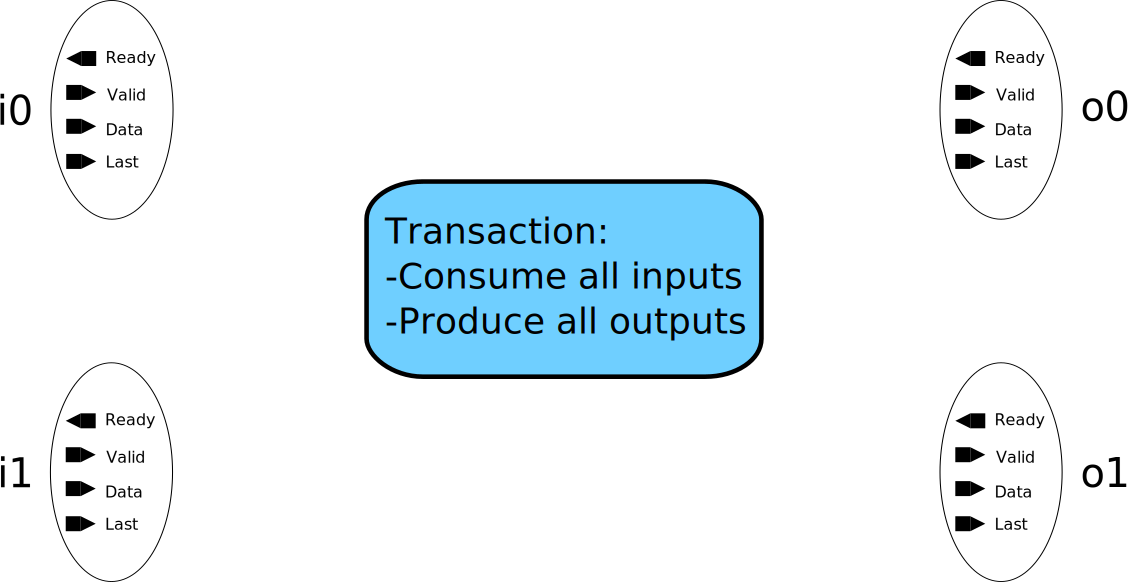
\includegraphics[width=\gwidth]{figs/sync_decoupled.svg}
  \end{figure}
  \small
\begin{verbatim}
SyncDecoupled(ins = ..., outs = ...)
\end{verbatim} 
\normalsize
\begin{itemize}
  \item Adds necessary control logic to graph
  \item More flexible than module-level reuse
\end{itemize}
\end{frame}

\begin{frame}[fragile]{Using Scala}
  % SyncDecoupled uses functional programming
  % Sample datatype uses operator overloading
  \small
\begin{verbatim}
sum_q.io.enq.bits := io.i0.bits + io.i1.bits
diff_q.io.enq.bits := io.i0.bits - io.i1.bits
\end{verbatim}
\normalsize
\begin{itemize}
\item Operator overloading makes this work
\item Performs add using built-in \texttt{Complex}'s \texttt{+}
\item \texttt{Complex} itself has overloaded operators
\end{itemize}
\end{frame}

\begin{frame}[fragile]{Using Scala}
  % SyncDecoupled uses functional programming
  % Sample datatype uses operator overloading
  \small
\begin{verbatim}
SyncDecoupled(ins = ..., outs = ...)
object SyncDecoupled {
  def apply(ins: Seq[DecoupledIO[Data]],
    outs: Seq[DecoupledIO[Data]]): Unit = {
    val allInsValid = ins.map(_.valid).reduce(_ && _)
    val allOutsReady = outs.map(_.ready).reduce(_ && _)
    for (in <- ins) {
      val otherInsValid =
        ins.filter(_ != in).map(_.valid).reduce(_ && _)
      in.ready := otherInsValid && allOutsReady
    }
    for (out <- outs) {
      val otherOutsReady =
        outs.filter(_ != out).map(_.ready).reduce(_ && _)
      out.valid := otherOutsReady && allInsValid
    }
  }
}
\end{verbatim}
\normalsize
\end{frame}

\begin{frame}{Does this imply a steep learning curve?}
  \begin{figure}
    \centering
    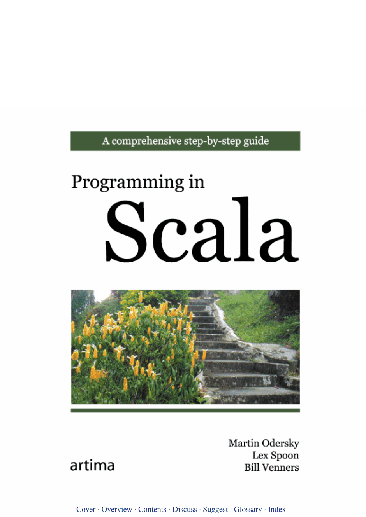
\includegraphics[width=0.4\textwidth]{images/programming-in-scala.pdf}
  \end{figure}
  \begin{itemize}
    \item Java-style OOP alone can unlock extreme capability
    \item<2-> We want to provide a library of powerful tools!
  \end{itemize}
\end{frame}

\begin{frame}{SDK: Powerful tools, simple interfaces}
  \begin{itemize}
  \item Library of components and patterns
  \item Simple use helps newcomers from Verilog
  \item Generality helps experienced users
  \item<2-> Identifying the patterns helps us!
    \begin{itemize}
    \item We're interested in the structure of DSP hardware
    \item Can we identify a basis for quickly building systems?
    \end{itemize}
  \end{itemize}
\end{frame}

\begin{frame}{Chisel can fit at any level}
  % Concentric circles changing color
  % Advantages at each level
\begin{columns}
  \begin{column}{0.4\textwidth}
    \begin{figure}
      \centering
      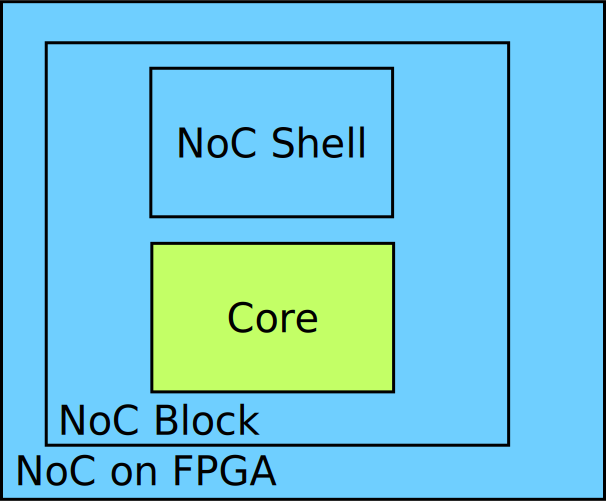
\includegraphics[width=\textwidth]{figs/chisel_2.svg}
    \end{figure}
  \end{column}
  \begin{column}{0.6\textwidth}
    Within the ``core logic'' of a block
    \begin{itemize}
      \item Easy to get started
      \item Library supports FIFO blocks
    \end{itemize}
  \end{column}
\end{columns}
\end{frame}

\begin{frame}{Chisel can fit at any level}
  % Concentric circles changing color
  % Advantages at each level
\begin{columns}
  \begin{column}{0.4\textwidth}
    \begin{figure}
      \centering
      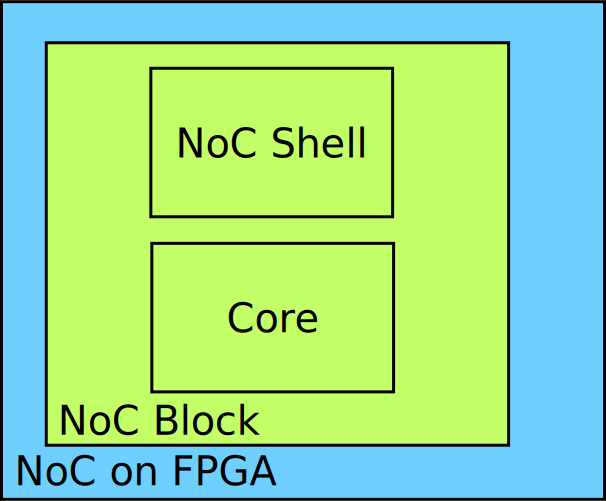
\includegraphics[width=\textwidth]{figs/chisel_3.svg}
    \end{figure}
  \end{column}
  \begin{column}{0.6\textwidth}
    Within an endpoint block
    \begin{itemize}
      \item NoC shell is highly parametrized -- Chisel helps
      \item Amortize work of ``language boundary crossings''
    \end{itemize}
  \end{column}
\end{columns}
\end{frame}

\begin{frame}{Chisel can fit at any level}
  % Concentric circles changing color
  % Advantages at each level
\begin{columns}
  \begin{column}{0.4\textwidth}
    \begin{figure}
      \centering
      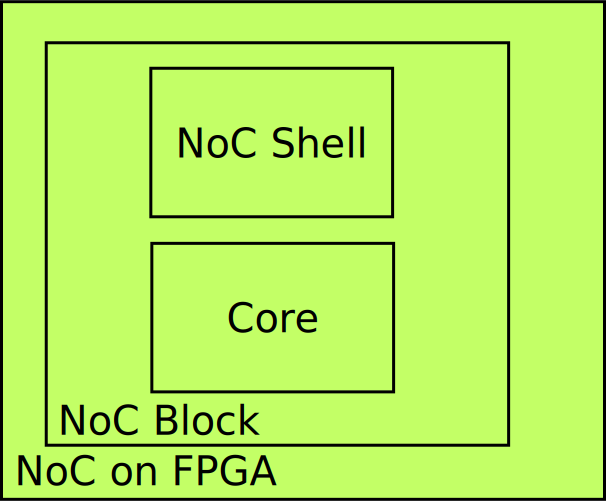
\includegraphics[width=\textwidth]{figs/chisel_4.svg}
    \end{figure}
  \end{column}
  \begin{column}{0.6\textwidth}
    Whole system RTL
    \begin{itemize}
      \item Chisel generators: flexible NoC configuration
      \item Parameters move easily though hierarchy
    \end{itemize}
  \end{column}
\end{columns}
\end{frame}

\begin{frame}{We're building solutions for DSP in software}
  \begin{figure}
    \centering
    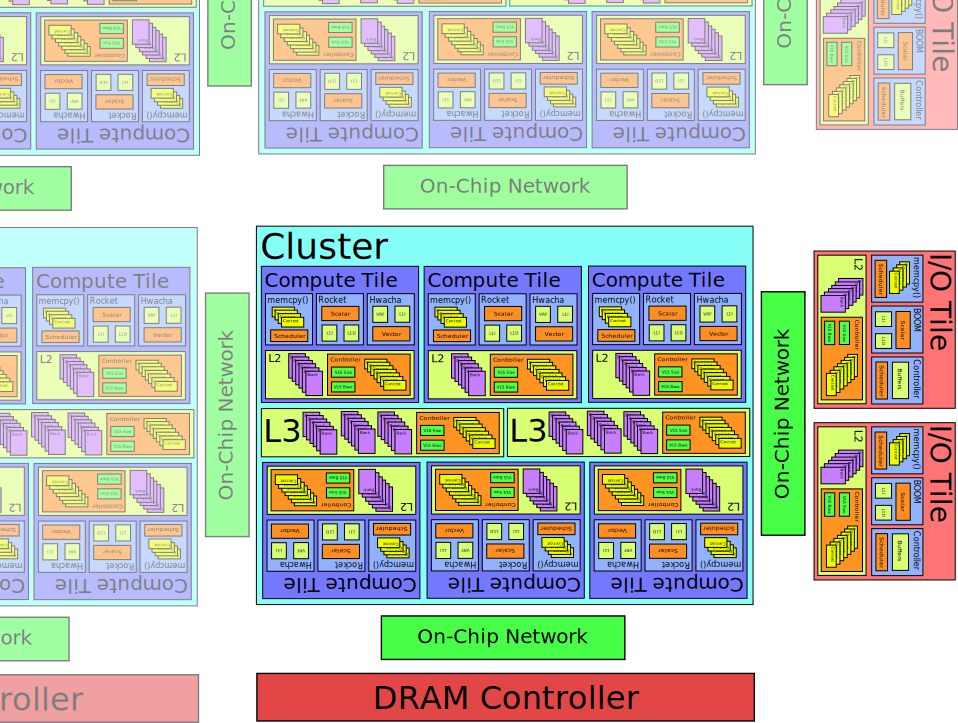
\includegraphics[width=0.4\textwidth]{figs/fabric.svg}
  \end{figure}
  \begin{itemize}
    \item Hurricane: a spatial array for DSP applications
    \item Aims to be better than past embedded manycores
      \begin{itemize}
        \item Better DLP with vector units
        \item Co-existance of implicit and explicit locality
        \item Support for cheap producer-consumer synchronization
        \item And more!
      \end{itemize}
  \end{itemize}
\end{frame}

\begin{frame}{We still like specialized hardware}
  \begin{figure}
    \centering
    \includegraphics[width=\textwidth]{figs/chisel.svg}
  \end{figure}
\end{frame}

\begin{frame}{Chisel above the RTL}
  \begin{itemize}
  \item We work in the hardware-software co-design space
  \item The USRP model is great
    \begin{itemize}
    \item GNU radio blocks stream across HW/SW
    \item Boundaries are handled abstractly
    \end{itemize}
  \item Where can Chisel fit in?
  \item How high-level of a system can it describe?
  \end{itemize}
\end{frame}

\end{document}
